\documentclass[12pt,fleqn]{article}\usepackage{../common}
\begin{document}
Ders 11

Bu ders oldukca teorik olacak ama icindeki fikirler bu derste ogretilen en
onemli fikirlerin arasinda. Su denklemi hatirlarsak

\[ y'' + p(x)y' + q(x)y = 0 \]

Bu denklemin cozum yontemi iki tane bagimsiz $y_1$ ve $y_2$ bulmaktan
geciyordu. Bagimsizligin tanimi mesela $y_2$'nin $y_1$'in ``kat�''
olmamas�, yani bir cozumu tamsayi bir sabitle carpinca digerini elde
edememeliyiz. Yani $y_2 \ne cy_1$, ve $y_1 \ne c'y_2$, ve $y_1 = 0$ ise
$y_2$ sifir olmamali. 

Usttekileri belirtmemizin sebebi neydi? Ki boylece ODE'nin tum cozumlerinin
$y_1$ ve $y_2$'nin bir lineer kombinasyonu oldugunu soyleyebilmek, yani

\[ y = c_1 y_1 + c_2 y_2 \]

Bu derste cevaplandiracagimiz soru �u: Niye? 

Soru 1: Niye $c_1 y_1 + c_2 y_2$'in hepsi bir cozumdur?

Bu soruyu bu dersteki ogrenciler cevaplayabilir herhalde, fakat temiz, oz,
zarif (elegant) bir sekilde cevaplayabilmek onemli olan ve aslinda bu
dersin de konusu. Bu cevabi oz, temiz bir sekilde veremezsek, daha ileride
daha cetrefil isleri halledemeyiz. 

1. soru lineer kombinasyonlarin niye cozum olduklarini cevaplayacak, fakat
``t�m'' cozumlerin onlar oldugunu daha zor olan 2. sorunun cevabi
belirleyecek.

Soru 2: Niye t�m cozumler bunlard�r?

Birinci sorunun cevabi ust uste eklenebilmek (superposition) prensibi
sayesinde cevaplanacak, ki bu prensip lineer kombinasyon argumaniyla ayni
sey. Ek bir not bu prensibin  ODE hangi dereceden olursa olsun (yani 2
oldugu gibi, 3, 4, vs. bile olabilir, form degismedigi surece derece
artabilir) prensibin gecerli olmasidir. 

Bu ispati yapmanin temiz yontemlerinden biri, azicik yol disina cikip
(detour), lineer operatorlerden bahsetmektir. Bu operatorleri dersimizin
geri kalaninda surekli kullanacagiz, onlari iyice tanimamiz iyi olur. 

Amacim ust uste eklenebilme prensibinin ispati, oraya gelirken, degisik
yerlere girip cikacagiz. Ana formu tekrar yazalim. 

\[ y'' + p(x)y' + q(x)y = 0 \]

Simdi bu formu turev alma operatorunu kullanarak tekrar yazacagim. Operator
$D$, bir kere turev al demektir, $D^2$ iki kere turev al demektir. O zaman

\[ D^2y + pDy + qy = 0  \]

$y$'yi disari cekelim

\[ (D^2 + pD + q)y = 0  \]

Burada dikkat: insanlar yukaridaki ibareyi ``parantez icinde bir seyler
{\em �arp�} y'' diye okumaya meyilli oluyor, bu dogru degil. Boyle bir ima
var gibi ama gercekte olan bu degil, cunku D operatoru y ``uzerinde'' islem
yapan bir operator. Aslinda usttekini yaparken amacim suydu, parantez
icindeki her seyi baslina basina tek bir operator haline cevirmek, ki bu
operatore $L$ adi verelim

\[ \underbrace{(D^2 + pD + q)}_{L}y = 0  \]

O zaman geriye 

\[ Ly = 0 \]

kalir. Formel olarak $L$'nin tanimi usttekidir, onu zihnimizde bir kutu
olarak ta canlandirabiliriz, kutuya bir fonksiyon giriyor, disari baska bir
fonksiyon cikiyor.

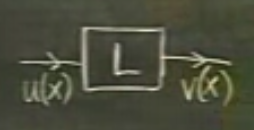
\includegraphics[height=2cm]{11_1.png}

Daha da detaylandirmak gerekirse, sayilar icin fonksiyonlar neyse,
fonksiyonlar icin operatorler o'dur. Bir fonksiyona sayi girer, disari sayi
cikar, bir operatore ise fonksiyon girer, bu fonksiyon degisime ugrayip
disari baska fonksiyon olarak cikar. Turev alma operatoru en basit
orneklerden biridir, mesela $x^2$ fonksiyonu turev operatoru $D$'ye girerse,
disariya yeni bir fonksiyon $2x$ cikar.

ODE'ye donersek, ustteki ODE'yi cozmek demek $L$ kutusundan sifir ciktigini
dusunmek ve bunun olmasi icin kutuya ne girdigini bulmaya calismak. Bir
ODE'yi cozmek, o zaman, bir tersine cevirme (inverse) problemidir. Tabii
ters yonde gitmek ileri yonde gitmekten daha zordur. 

Bu operatorun lineer oldugunu hatirlayalim. Bu, operator fonksiyonlarla
is gordugu zaman belli ozellikler gosterir. 

\[ L(u_1 + u_2) = L(u_1) + L(u_2) \]

\[  L(cu) = cL(u)\]

ki $c$ bir sabit, $u$, $u_1$ ve $u_2$ fonksiyonlardir. 

Ustteki iki ifade lineerligin iki kuralidir. Bu kurallar normal
fonksiyonlar icin de gecerlidir bu arada. 

Ornek? $D$ operatoru lineer bir operatordur. Cunku, mesela

\[ (u_1 + u_2)' = u_1' + u_2' \]

\[ (cu)' = cu' \]

Bu Calculus dersinden bildigimiz bir sey. Yani en temel Calculus'tan
beri bildigimiz ustteki kurallar aslinda $D$ operatorunun lineer bir
operator oldugunun da gostergesidir.

Not: Ya peki carpma? O da bir sekilde duruma dahil mi? Onun da kullanildigi
bazi durumlar var ama lineerlik baglaminda konumuzun disinda.

Neyse, tum bu kurallari ust uste eklenebilme prensibini ispatlayabilmek
icin ortaya koyduk, simdi ispatin kendisine gelelim. 

Teori

ODE'miz soyle:

\[ Ly = 0 \]

Eger $y_1$ ve $y_2$ cozum ise alttaki de bir cozumdur.

\[ y = c_1 y_1 + c_2 y_2 \]

Ispat

$L$ operatorunu ustteki kombinasyona uygulayalim:

\[ L(c_1 y_1 + c_2 y_2) = L(c_1 y_1) + L(c_2 y_2)\]

\[ = c_1L(y_1) + c_2L(y_2)\]

Simdi yapmaya calistigim bunu sifir oldugunu gostermek. Eger $y_1$ bir
cozum ise o zaman $Ly=0$'dan hareketle $L(y_1)$'in sifir olmasi
gerekir. Ayni sekilde $L(y_2) = 0$.

\[ = c_1 \cdot 0 + c_2 \cdot 0 = 0 \]

Ispat tamamlandi. Bu argumani ODE'nin orijinal formunu kullanarak ta
yapabilirdik tabii, ama o zaman degiskenleri yerine koyup, cebirsel
gruplama yapacak, bir suru islem icine girecektik. Bu bize sonucu
verecekti, ama ispatin niye boyle sonuc verdigini acik bir sekilde
soylemeyecekti. Ispat basarili oldu cunku $L$ bir lineer operatordu. 

Simdi daha zor olan ikinci soruya gelelim. Bu soruyu cevaplayacagiz, ama
bir yan yola girerek, cevabi ``baslangic deger problemini cozme'' a��s�ndan
anlamaya ugrasacagiz, baslangic degerlerini formule uydurarak (fitting) bir
yere gelmeye cabalayacagiz. 

Teori

Tum lineer kombinasyonlari bir kume olarak dusunelim, 

\[ \bigg\{ c_1y_1 + c_2y_2 \bigg\} \]

Bana hangi baslangic degerini verirsen verin, bu kume icinde ona uygun bir
$c_1$ ve $c_2$ bulabilirim. 

Ispat

Bu ispati yaparken simdiye kadar ODE cozerken odevlerde gelistirdigimiz
baslangic degerlerini kullanip sabitleri hesaplama becerisinden
faydalanacagiz, ama sayilar yerine semboller kullanacagiz. Diyelim ki 

\[ y(x_0) = a \]

\[ y(x_0) = b \]

Yerine koyarsak

\[ y = c_1y_1 + c_2y_2 \]

\[ y' =  c_1y_1' + c_2y_2'\]

$x=x_0$'i yerine koyalim

\[ y = c_1y_1(x_0) + c_2y_2(x_0) = a\]

\[ y' =  c_1y_1'(x_0) + c_2y_2'(x_0) = b\]

Odev problemlerinde $y_1$ ve $y_2$ somut fonksiyonlar oluyordu, $e^x$ gibi
mesela. Burada sadece onun yerine sembolik degerler kullaniyorum. 

Simdi ustteki iki denkleme bakalim. Bu bir beraber cozulecek (simultaneous)
lineer denklem sistemi degil midir? Cozulecek, bulunacak degiskenler
hangileri? $c_1$ ve $c_2$. Buna tam aliskin degiliz, genellikle cozulecek
degiskenler terimlerin onunde degil arkasinda olur, ustelik $c_1$ ve $c_2$
simdiye kadar hep ``sabit'' olarak etiketledigimiz seyler, ama biraz daha
dusunursek ve geri kalan arap saci gibi terimlere dikkatlice bakarsak
lineer sistemi gorebiliriz. Bu sistemde degiskenler $c_1$ ve $c_2$. 

Peki simdi su soruyu soralim. Ustteki sistemin ne zaman bir cozumu vardir?
Sistem her zaman cozulemeyebilir. Cevap: Eger katsayi matrisinin tersi
alinabiliyor ise (invertible), yani matrisin determinanti sifir haricinde
bir deger olmali. 

\[ 
\left|\begin{array}{rr}
y_1 & y_2 \\
y_1' & y_2'
\end{array}\right|_{x_0}
\ne 0
 \]

Determinant isareti $|$'nin alt kosesindeki $x_0$, matris icindeki tum
fonksiyonlarin $x_0$ verilerek elde edilen sonuclarini kullanmamiz
gerektigini soyluyor.  

Ustteki determinant onemli bir determinant, ve bir ismi var:
Wronskian. Sembolik kullanimi ise soyle: $W(y_1, y_2)$. Hepsini bir arada
belirtirsek, 

\[ W(y_1, y_2) = 
\left|\begin{array}{rr}
y_1 & y_2 \\
y_1' & y_2'
\end{array}\right|
 \]

Wronskian'i ona gecilen iki fonksiyonu biliyorsak hesaplayabiliriz, ama
$W$, $y_1$ ve $y_2$'nin fonksiyonu degil. Wronskian $x$'in bir fonksiyonu
aslinda. 

Wronskian'in sifir olmama durumunu nasil ispatlariz? Diyelim ki $y_2$ ve
$y_1$ birbirine bagimli (dependent), yani $y_2 = cy_1$. Bunun boyle
olmadigini biliyoruz cunku ODE'nin farkli cozumleri var. Ama oldugunu
dusunelim, ve ustteki determinanta bakalim, $y_2 = cy_1$ olmasi ne
demektir?  $y_2' = cy_1'$ sartinin da gecerli olmasi demektir. Ve bu sart
gerceklesirse, o zaman Wronskian, her $x$ degeri icin, her zaman,
kesinlikle sifir olacaktir, cunku artik iki kolon tamamen birbirinin kati
haline gelmistir.

Odev sorularinda ogrencinin ispatlamasini istedigimiz teori bu. 

Teori

Eger $y_1$ ve $y_2$ ODE'mizin cozumu ise, o zaman sadece iki secenekten
biri dogru olabilir. Ya her $x$ degeri icin $W(y_1,y_2) = 0$ (aslinda her
$x$ degeri icin sozu fazlalik, cunku Wronskian tanimi zaten o ifadeyi
kapsiyor, ama bu bir giris dersi oldugu icin tekrarliyoruz), ya da
Wronskian hicbir zaman sifir degil.

Simdi, bir parantez daha aciyoruz. Bu ikinci parantez de kapaninca, ustteki
``2. sorunun'' cevabini vermek icin elimizde tum gerekli araclar olacak. 

Yukarida ODE cozumunun tum cozumlerinin surada oldugunu belirtmistik

\[ \bigg\{ c_1y_1 + c_2y_2 \bigg\} \]

Onemli nokta su ki, $y_1$ ve $y_2$ oyle ``ozel'', ``kutsal'' cozumler
degiller. Sunu da soyleyebilirdik ve ustteki ifade ile ayni sey olurdu

\[ \bigg\{ c_1'u_1 + c_2'u_2 \bigg\} \]

ki $u_1$ ve $u_2$ herhangi baska bir lineer olarak bagimsiz cozumler. 

Bunu niye soyledik? $y_1$ ve $y_2$ genelde denklemi cozdugumuz zaman elde
ettigimiz kolay cozumlerdir, mesela $e^x$, $e^2x$, $\cos(x)$,
vs. turunde. Cozumu bu tur ogeleri kullanarak yazmak bir yontem tabii,
fakat tek yontem degil. Bazi ODE'ler icin ``normalize edilmis cozumler''
bulmak daha iyi. 

Normalize edilmis cozumler belli bazi ozel baslangic sartlarini tatmin eden
cozumlerdir. Eger $Y_1$ ve $Y_2$'yi normalize edilmis cozumler olarak kabul
edersek, bu sartlar

\[ Y_1(0) = 1, \  Y_2(0) = 0 \  \]

\[ Y_1'(0) = 0, \  Y_2'(0) = 1 \  \]

Ornek 

\[ y'' + y = 0 \]

Standart cozumler $y_1 = \cos(x)$, $y_2 = \sin(x)$. $y_1$'in 0'daki degeri
nedir? 1. $y_1'$'in sifirdaki degeri nedir? 0. Demek ki $y_1$ normalize
edilmis, yani $Y_1$. $y_2$ ayni sekilde $Y_2$ olur. 

Not: Normalize cozumleri cogunlukla bir bakista bu kadar kolay goremiyoruz
tabii ki. 

Ornek 

\[ y'' - y = 0 \]

Karakteristik denklemler 1, ve -1, o zaman cozum $y_1 = e^x$ ve $y_2 =
e^{-x}$. 
Genel cozum 

\[ y = c_1 e^x + c_2 e^{-x} \]

Buradan normalize cozumleri, mesela $Y_1$, nasil buluruz? Baslangic
sartlarini yerine getirerek. Bu arada $y'$

\[ y' = c_1 e^x - c_2 e^{-x} \]

Sartlari koyalim. $y_1(0)$

\[ c_1 + c_2 = 1 \]

$y_1'(0)$

\[ c_1 - c_2 = 0 \]

Bu bir denklem sistemi yaratti, o zaman $c_1 = c_2 = 1/2$. O zaman 

\[ Y_1 = \frac{e^x + e^{-x}}{2} \]

$Y_2$'yi benzer sekilde buluruz, hesaplari yaptiktan sonra sonuc

\[ Y_2 = \frac{e^x - e^{-x}}{2} \]

cikacaktir. Yani ornek ODE'miz icin bu iki cozum normalize edilmis
cozumlerdir. Bu cozumler asil cozumlerden ``daha iyi'', cunku baslangic
sartlari daha ``guzel''. Cozume ve turevini sifir noktasinda hesaplayinca
bunu goruyoruz, sonuc ya 0 ya da 1 geliyor. Temiz. Bu arada bu ornekte elde
ettigimiz $Y_1$, $cosh(x)$ (hiperbolik kosinus) ve $Y_2$, $sinh(x)$
(hiperbolik sinus) olarak bilinir. 

Muhendisler normalize cozumler cok severler, cunku eger $Y_1$ ve $Y_2$
sifirda normalize edilmisse, o zaman baslangic deger problemi, yani bizim
klasik ODE'miz arti

\[ y(0) = y_0 \]

\[ y'(0) = y_0' \]

denkleminin cozumu soyledir

\[ y = y_0 Y_1 + y_0' Y_2 \]

Diger bir deyisle, eger bir denklemin normalize cozumlerini bulmussak /
biliyorsak, genel cozum icin baslangic sartlarini {\em oldugu gibi} alip
genel cozumu yaratmak icin kullanabiliriz. 

Ustteki $y$'nin dogru olup olmadini kontrol edebilirsiniz. Mesela $y(0)$
nedir? O noktada $Y_1(0)=1$, $Y_2(0)=0$ olduguna gore  $y(0)=y_0$ elde
ederiz, ki bu ustteki baslangic sartlari ile uyar. Geri kalanini siz
kontrol edebilirsiniz. 

Boylece ikinci parantezi kapattik. Artik ``buyuk teori'' icin gereken her
sey var.

Mevcudiyet ve Ozgunluk Teorisi (Existence and Uniqueness Theorem)

Standart ODE

\[ y'' + py' + qy = 0 \]

oyle ki $p$ ve $q$ her $x$ icin surekli fonksiyonlar (``iyi'' fonksiyonlar
yani, katsayilar hicbir noktada patlamiyor). 

O zaman, bu teoriye gore, verilen baslangic sartlari

\[ y(0) = A \]

\[ y'(0) = B \]

uyumlu bir cozumu, ve sadece bir tane cozum vardir. 

Bir cozum olmasi teorinin ``mevcudiyet'' tarafi, o cozumun tek mumkun cozum
olmasi teorinin ozgunluk tarafi. 

Iddia ediyorum ki 

\[ \bigg\{ c_1Y_1 + c_2Y_2 \bigg\} \]

kumesi tum cozumleri iceriyor. 

Ispat

Verilen herhangi (arbitrary) bir cozum $u(x)$, ki

\[ u(0) = u_0 \]

\[ u'(0) = u_0' \]

alinip su sekilde kullanilinca

\[ u_0 Y_1 +  u_0'Y_2 \]

bu ifade baslangic sartlariyla uyumlu olur. 


\end{document}

